\section{A complete example: from shared values to counting tables}
\label{sec:counting-walkthrough}

The algorithm's basic question is what must remain known after part of a
circuit has been processed. An accepting input determines every gate value,
but a partial calculation must retain the values on which unprocessed gates
still depend. We work through this distinction numerically before using
graph width to bound the size of those partial calculations.

The organizing principle is that a processed region interacts with the
remaining circuit only through their shared values. A table indexed by
those values can therefore replace the region, recording the number of
compatible internal assignments in each entry. Internal assignments with
the same boundary values have identical effects on every remaining
constraint. Their identities can be discarded while their multiplicity
is retained. This conditional-count interpretation will serve as the
invariant of both local elimination and frontier evaluation.

\subsection{Gate equations preserve the objects being counted}

Return to the circuit
\[
 v_1=x\lor y,\qquad v_2=y\oplus z,\qquad
 v_3=v_1\land v_2,\qquad f(x,y,z)=v_3.
\]
Here all three inputs are quantified when we count satisfying assignments.
The symbols $v_i$ denote gate values; the parameter $b$ elsewhere still
denotes the number of retained inputs. Introduce indicator tables
\[
 \begin{aligned}
 G_1(x,y,a)&=[a=x\lor y],&
 G_2(y,z,c)&=[c=y\oplus z],\\
 G_3(a,c,d)&=[d=a\land c],& O(d)&=[d=1].
 \end{aligned}
\]
Brackets equal one when their statement holds and zero otherwise. The
letters $a,c,d$ are possible values of $v_1,v_2,v_3$, respectively.
The exact count is
\begin{equation}\label{eq:walk-count}
 Z=\sum_{x,y,z,a,c,d\in\B}
 G_1(x,y,a)G_2(y,z,c)G_3(a,c,d)O(d).
\end{equation}
Why does this sum count inputs, although it also sums over gate values?
For each fixed $(x,y,z)$, the first equation forces $a$, the second forces
$c$, and the third then forces $d$. There is exactly one extension satisfying
the three gate equations. The output factor keeps that extension exactly
when the input accepts. Thus the extra variables introduce no multiplicity.
This topological argument is the step needed for counting; preservation of
mere satisfiability would not suffice.

The complete evaluation table makes this bijection visible:
\[
\begin{array}{ccc|ccc}
 x&y&z&v_1&v_2&v_3\\ \hline
 0&0&0&0&0&0\\
 0&0&1&0&1&0\\
 0&1&0&1&1&1\\
 0&1&1&1&0&0\\
 1&0&0&1&0&0\\
 1&0&1&1&1&1\\
 1&1&0&1&1&1\\
 1&1&1&1&0&0
\end{array}
\]
The accepting triples are $010,101,110$, so $Z=3$. If $x$ is ordinary
and $(y,z)$ are witnesses instead, the witness counts are $1$ and $2$,
while both ordinary inputs have an accepting witness. Counting accepting
pairs gives three; counting distinct positive projected inputs gives two.

\subsection{Why a directed acyclic circuit has a consistency cycle}

The incidence graph has a vertex for each of the six values
$x,y,z,v_1,v_2,v_3$, and a vertex for each of $G_1,G_2,G_3,O$.
An edge records a value's occurrence in a table. Thus each gate table has
three incident edges and $O$ has one: there are ten vertices and ten edges.
The graph is connected. For a connected graph, its \emph{cycle rank}
$|E|-|V|+1$ counts the edges left after a spanning tree is removed.
Here the cycle rank is $10-10+1=1$.

\begin{figure}[htbp]
\centering
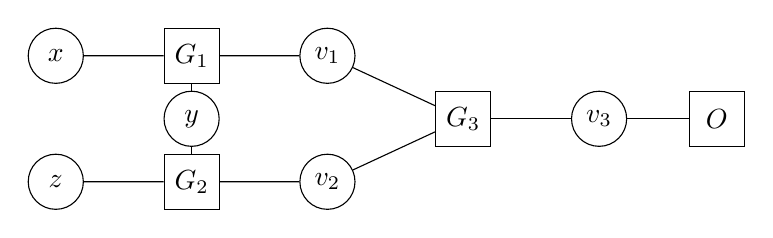
\begin{tikzpicture}[x=1.15cm,y=0.8cm,
 value/.style={circle,draw,minimum size=7mm,inner sep=1pt},
 factor/.style={rectangle,draw,minimum size=7mm,inner sep=2pt}]
 \node[value] (x) at (0,1) {$x$};
 \node[factor] (g1) at (1.5,1) {$G_1$};
 \node[value] (a) at (3,1) {$v_1$};
 \node[value] (y) at (1.5,0) {$y$};
 \node[value] (z) at (0,-1) {$z$};
 \node[factor] (g2) at (1.5,-1) {$G_2$};
 \node[value] (c) at (3,-1) {$v_2$};
 \node[factor] (g3) at (4.5,0) {$G_3$};
 \node[value] (d) at (6,0) {$v_3$};
 \node[factor] (o) at (7.3,0) {$O$};
 \draw (x)--(g1)--(a)--(g3)--(c)--(g2)--(z);
 \draw (g1)--(y)--(g2);
 \draw (g3)--(d)--(o);
\end{tikzpicture}
\caption{Circles enforce agreement between occurrences of one value;
rectangles enforce gate equations or the output condition. The cycle runs
through $y,G_1,v_1,G_3,v_2,G_2$.}
\label{fig:walk-incidence}
\end{figure}

There is no directed feedback in the original circuit. The undirected cycle
records two uses of $y$ whose branches later meet at $G_3$. This is precisely
the agreement a local calculation must preserve. In the all-quantified
notation of Lemma~\ref{lem:consistency-budget}, $q=b=3$, $h=0$, and
$\ell=6$, giving $\kappa=6-3-3+1=1$ and $h+b+\kappa=q+1=4$.

To obtain a network of small tables, give each incidence edge its own bit.
At every circle of degree $D$, put the equality table
\[
 E_D(t_1,\ldots,t_D)=[t_1=\cdots=t_D].
\]
Here $E_1(0)=E_1(1)=1$: a leaf input is free, not fixed to one.
At each rectangle put its indicated gate or output table. Sum the product
of all these tables over the ten edge bits. A nonzero product requires all
copies of each value to agree. Each assignment satisfying the gate equations
then determines exactly one assignment to all ten edges, and conversely.
Consequently this edge-index sum is also $Z$.

An array with one coordinate per incident edge is called a tensor. Its
contraction sums products over shared coordinates. This is the standard
tensor-network perspective on circuit simulation \citep{MarkovShi2008};
the elementary zero-one correspondence above establishes the particular
counting interpretation needed here.

\subsection{Eliminate two inputs and inspect every surviving entry}

First sum over $x$ and $z$, retaining the common value $y$:
\[
 A(y,a)=\sum_x [a=x\lor y],\qquad
 B(y,c)=\sum_z [c=y\oplus z].
\]
Rows are indexed by $y=0,1$ and columns by the indicated gate value $0,1$:
\begin{equation}\label{eq:walk-matrices}
 A=\begin{pmatrix}1&1\\0&2\end{pmatrix},\qquad
 B=\begin{pmatrix}1&1\\1&1\end{pmatrix}.
\end{equation}
For $y=0$, exactly one $x$ produces each possible OR output. For $y=1$,
neither $x$ produces output zero and both produce output one; this explains
the entry two. For each fixed $y$ and XOR output $c$, exactly one $z$
works, explaining all four ones in $B$.

Next sum over $d$. The output must be one, so
\[
 C(a,c)=\sum_d[d=a\land c][d=1]=[a=c=1].
\]
The remaining sum collapses to
\begin{equation}\label{eq:walk-three}
 Z=\sum_{y,a,c}A(y,a)B(y,c)C(a,c)
  =\sum_y A(y,1)B(y,1)=1\cdot1+2\cdot1=3.
\end{equation}
The first term represents $101$; the second represents $010$ and $110$.
What would happen if the two uses of $y$ were independently summed away?
The result would instead be
\[
 \left(\sum_y A(y,1)\right)
 \left(\sum_{y'}B(y',1)\right)=(1+2)(1+1)=6.
\]
This counts assignments to a changed circuit with two independent inputs
in place of the shared $y$. The extra three combinations disagree between
the two branches. The equality table prevents precisely those combinations.

The same counting rule applies when the local operation changes.
Replacing the XOR gate by AND gives
\[
 B_{\land}=\begin{pmatrix}2&0\\1&1\end{pmatrix},
 \qquad Z=1\cdot0+2\cdot1=2.
\]
The surviving inputs are $011$ and $111$. The local table changes;
the requirement to retain one shared $y$ does not.

Pinning $x$ exposes the two witness fibers without changing the network's
edges. Replace its leaf table $(1,1)$ by $(1,0)$ for $x=0$ or $(0,1)$
for $x=1$. The resulting left tables are
\[
 A_{x=0}=\begin{pmatrix}1&0\\0&1\end{pmatrix},\qquad
 A_{x=1}=\begin{pmatrix}0&1\\0&1\end{pmatrix}.
\]
Equation~\eqref{eq:walk-three} now gives $0+1=1$ and $1+1=2$.
Further pins give $Z_{x=0,y=0}=0$, $Z_{x=0,y=1}=1$, and
$Z_{x=1,y=0}=Z_{x=1,y=1}=1$. A pin is evidence restricting an original
input, not an additional independent choice.

\subsection{The same operations answer existence and counting}

For decision, replace every sum by OR and every product by AND. An
intermediate entry now says whether at least one internal assignment works,
rather than how many work. This is calculation in the Boolean semiring
$(\B,\lor,\land)$; counting uses the nonnegative-integer semiring
$(\mathbb{N},+,\cdot)$. Both support distributivity, so the same contraction
identities apply. In particular, the entry two of $A$ becomes one under
Boolean contraction. Thresholding a nonnegative integer count at zero
commutes with both operations:
\[
 [r+s>0]=[r>0]\lor[s>0],\qquad
 [rs>0]=[r>0]\land[s>0].
\]
For fixed ordinary $x$, the Boolean result is
$g(x)=\bigvee_{y,z}f(x,y,z)$ and the integer result is
$W(x)=\sum_{y,z}f(x,y,z)$. Hence $g(x)=[W(x)>0]$.
Counting projected inputs requires $\sum_x[W(x)>0]$, which is not
$\sum_x W(x)$. A sum-product calculation over all original inputs computes
the latter. There is no automatic projected-counting guarantee from merely
changing OR into addition.

An ordinary input can also remain symbolic throughout the calculation.
For a separate small example, take
\[
 \psi(x_1,x_2;y)=(x_1\land y)\lor(x_2\land\neg y).
\]
Fixing $y=0$ kills the first term and leaves $x_2$; fixing $y=1$
kills the second and leaves $x_1$. The table indexed by $y$ therefore
contains the two circuit wires $x_2,x_1$, rather than two evaluated bits.
Boolean contraction of that index gives
\begin{equation}\label{eq:walk-symbolic}
 \bigvee_{y\in\B}\psi(x_1,x_2;y)=x_2\lor x_1.
\end{equation}
One OR gate connects these wires and works for all four ordinary inputs;
constructing it does not require enumerating those inputs. By comparison,
the integer witness count is $x_2+x_1$, which is two at $(x_1,x_2)=(1,1)$
although the Boolean projection is one. In the general symbolic construction,
each table entry similarly points to a circuit computing a Boolean function
of the ordinary inputs. OR and AND combine those pointers by adding gates.
When all original inputs are quantified for SAT, no ordinary-input wires
remain symbolic, and the tables instead have constant Boolean or integer
entries as in the running example.

Two small identities explain why multigraph details also matter. If two
ports of one table are joined by a loop, both ports carry the same bit.
For the two-port table
\[
 L=\begin{pmatrix}2&3\\5&7\end{pmatrix},
\]
closing the loop gives $L(0,0)+L(1,1)=9$, not the sum $17$ of all entries.
For two tables joined by two parallel edges, take
\[
 U=\begin{pmatrix}1&2\\3&4\end{pmatrix},\qquad
 V=\begin{pmatrix}5&6\\7&8\end{pmatrix}.
\]
Joint contraction gives $\sum_{r,s}U(r,s)V(r,s)=5+12+21+32=70$.
Contracting just the $r$ edge first gives
\[
 W(s,t)=\sum_r U(r,s)V(r,t)
       =\begin{pmatrix}26&30\\38&44\end{pmatrix}.
\]
The remaining edge becomes a loop, so its diagonal sum is again $70$.
Allowing its ends to vary independently would give $138$. These are local
integer-table fixtures, not additional gates of the running circuit.

\subsection{What the frontier remembers in a larger instance}

The example above reduces completely by the low-degree operations of
Lemma~\ref{lem:cubic-reduction}; its reduced cubic graph is empty. Indeed,
a nonempty connected cubic remainder would have cycle rank at least two,
whereas the initial graph has rank one and reductions cannot increase it.
The example demonstrates consistency and exact counting. It cannot test the
asymptotic pathwidth theorem that handles nonempty cubic remainders.

For that next stage, order the vertices of a reduced graph. After processing
a prefix, the \emph{frontier} consists of the edges with one processed and
one unprocessed endpoint. If there are $w_i$ such edges, the table has
$2^{w_i}$ entries. Each entry counts assignments to edges entirely inside
the processed region, conditioned on the frontier bits. The unprocessed
region has contributed no constraints yet. Thus a positive entry need not
extend to a solution of the whole instance.

At the next vertex, write $J$ for its edges into the processed region,
$R$ for its edges into the future, and $S$ for frontier edges not incident
to it. The old frontier is $S\cup J$ and the new one is $S\cup R$.
For its local table $T$, the update is
\begin{equation}\label{eq:walk-frontier}
 P_{i+1}(\sigma,\rho)=
 \sum_{\eta\in\B^J}P_i(\sigma,\eta)T(\eta,\rho).
\end{equation}
Every extension of the new boundary has a unique choice of the consumed
bits $\eta$ and a unique assignment counted by the corresponding old
entry. This proves the invariant by induction, starting with the empty
prefix's scalar one. At the end the boundary is empty and its scalar is
the desired count.

The product in the update combines assignments in disjoint regions with
matching consumed bits. The sum combines disjoint cases for those bits,
while the unchanged frontier remains fixed. Thus the algebra expresses
the conditional-count interpretation directly: a value is eliminated
only after all its incident constraints have been included in the
processed region.

For a concrete transition with two consumed edges and one new edge,
let $P_i(p,q)$ have rows $(1,2)$ and $(3,4)$, and let
$T(p,q,r)=[r=p\oplus q]$. There are no spectator edges. The new table is
$P_{i+1}(0)=1+4=5$ and $P_{i+1}(1)=2+3=5$. The old four entries are
summarized by two entries indexed by the value still needed in the future.
This standalone transition illustrates a cubic vertex update without
claiming that this particular table arose from our three-gate example.

The maximum frontier size of an order is its cutwidth. It controls table
storage and arithmetic operation counts. It is not by itself a bit-time
bound: integer entries also have a bit length. In the general construction
there are $O(s+1)$ edge indices, so an entry counts at most
$2^{O(s+1)}$ internal assignments and has $O(s+1)$ bits. Polynomial-cost
exact integer arithmetic then converts the contraction bound to the bit
bound proved in Corollary~\ref{cor:gate-counting}. The exponential table
storage is allowed there. The accompanying exhaustive script checks the
numbers, unique extensions, pins, and local contraction identities in this
section; it implements neither the full SAT solver nor its layout theorem.
